\PassOptionsToPackage{unicode=true}{hyperref} % options for packages loaded elsewhere
\PassOptionsToPackage{hyphens}{url}
%
\documentclass[11pt,ignorenonframetext,]{beamer}
\usepackage{pgfpages}
\setbeamertemplate{caption}[numbered]
\setbeamertemplate{caption label separator}{: }
\setbeamercolor{caption name}{fg=normal text.fg}
\beamertemplatenavigationsymbolsempty
% Prevent slide breaks in the middle of a paragraph:
\widowpenalties 1 10000
\raggedbottom
\setbeamertemplate{part page}{
\centering
\begin{beamercolorbox}[sep=16pt,center]{part title}
  \usebeamerfont{part title}\insertpart\par
\end{beamercolorbox}
}
\setbeamertemplate{section page}{
\centering
\begin{beamercolorbox}[sep=12pt,center]{part title}
  \usebeamerfont{section title}\insertsection\par
\end{beamercolorbox}
}
\setbeamertemplate{subsection page}{
\centering
\begin{beamercolorbox}[sep=8pt,center]{part title}
  \usebeamerfont{subsection title}\insertsubsection\par
\end{beamercolorbox}
}
\AtBeginPart{
  \frame{\partpage}
}
\AtBeginSection{
  \ifbibliography
  \else
    \frame{\sectionpage}
  \fi
}
\AtBeginSubsection{
  \frame{\subsectionpage}
}
\usepackage{lmodern}
\usepackage{amssymb,amsmath}
\usepackage{ifxetex,ifluatex}
\usepackage{fixltx2e} % provides \textsubscript
\ifnum 0\ifxetex 1\fi\ifluatex 1\fi=0 % if pdftex
  \usepackage[T1]{fontenc}
  \usepackage[utf8]{inputenc}
  \usepackage{textcomp} % provides euro and other symbols
\else % if luatex or xelatex
  \usepackage{unicode-math}
  \defaultfontfeatures{Ligatures=TeX,Scale=MatchLowercase}
\fi
\usetheme[]{metropolis}
% use upquote if available, for straight quotes in verbatim environments
\IfFileExists{upquote.sty}{\usepackage{upquote}}{}
% use microtype if available
\IfFileExists{microtype.sty}{%
\usepackage[]{microtype}
\UseMicrotypeSet[protrusion]{basicmath} % disable protrusion for tt fonts
}{}
\IfFileExists{parskip.sty}{%
\usepackage{parskip}
}{% else
\setlength{\parindent}{0pt}
\setlength{\parskip}{6pt plus 2pt minus 1pt}
}
\usepackage{hyperref}
\hypersetup{
            pdftitle={Lecture 1},
            pdfauthor={Colin Rundel},
            pdfborder={0 0 0},
            breaklinks=true}
\urlstyle{same}  % don't use monospace font for urls
\newif\ifbibliography
\usepackage{color}
\usepackage{fancyvrb}
\newcommand{\VerbBar}{|}
\newcommand{\VERB}{\Verb[commandchars=\\\{\}]}
\DefineVerbatimEnvironment{Highlighting}{Verbatim}{commandchars=\\\{\}}
% Add ',fontsize=\small' for more characters per line
\newenvironment{Shaded}{}{}
\newcommand{\AlertTok}[1]{\textcolor[rgb]{1.00,0.00,0.00}{\textbf{#1}}}
\newcommand{\AnnotationTok}[1]{\textcolor[rgb]{0.38,0.63,0.69}{\textbf{\textit{#1}}}}
\newcommand{\AttributeTok}[1]{\textcolor[rgb]{0.49,0.56,0.16}{#1}}
\newcommand{\BaseNTok}[1]{\textcolor[rgb]{0.25,0.63,0.44}{#1}}
\newcommand{\BuiltInTok}[1]{#1}
\newcommand{\CharTok}[1]{\textcolor[rgb]{0.25,0.44,0.63}{#1}}
\newcommand{\CommentTok}[1]{\textcolor[rgb]{0.38,0.63,0.69}{\textit{#1}}}
\newcommand{\CommentVarTok}[1]{\textcolor[rgb]{0.38,0.63,0.69}{\textbf{\textit{#1}}}}
\newcommand{\ConstantTok}[1]{\textcolor[rgb]{0.53,0.00,0.00}{#1}}
\newcommand{\ControlFlowTok}[1]{\textcolor[rgb]{0.00,0.44,0.13}{\textbf{#1}}}
\newcommand{\DataTypeTok}[1]{\textcolor[rgb]{0.56,0.13,0.00}{#1}}
\newcommand{\DecValTok}[1]{\textcolor[rgb]{0.25,0.63,0.44}{#1}}
\newcommand{\DocumentationTok}[1]{\textcolor[rgb]{0.73,0.13,0.13}{\textit{#1}}}
\newcommand{\ErrorTok}[1]{\textcolor[rgb]{1.00,0.00,0.00}{\textbf{#1}}}
\newcommand{\ExtensionTok}[1]{#1}
\newcommand{\FloatTok}[1]{\textcolor[rgb]{0.25,0.63,0.44}{#1}}
\newcommand{\FunctionTok}[1]{\textcolor[rgb]{0.02,0.16,0.49}{#1}}
\newcommand{\ImportTok}[1]{#1}
\newcommand{\InformationTok}[1]{\textcolor[rgb]{0.38,0.63,0.69}{\textbf{\textit{#1}}}}
\newcommand{\KeywordTok}[1]{\textcolor[rgb]{0.00,0.44,0.13}{\textbf{#1}}}
\newcommand{\NormalTok}[1]{#1}
\newcommand{\OperatorTok}[1]{\textcolor[rgb]{0.40,0.40,0.40}{#1}}
\newcommand{\OtherTok}[1]{\textcolor[rgb]{0.00,0.44,0.13}{#1}}
\newcommand{\PreprocessorTok}[1]{\textcolor[rgb]{0.74,0.48,0.00}{#1}}
\newcommand{\RegionMarkerTok}[1]{#1}
\newcommand{\SpecialCharTok}[1]{\textcolor[rgb]{0.25,0.44,0.63}{#1}}
\newcommand{\SpecialStringTok}[1]{\textcolor[rgb]{0.73,0.40,0.53}{#1}}
\newcommand{\StringTok}[1]{\textcolor[rgb]{0.25,0.44,0.63}{#1}}
\newcommand{\VariableTok}[1]{\textcolor[rgb]{0.10,0.09,0.49}{#1}}
\newcommand{\VerbatimStringTok}[1]{\textcolor[rgb]{0.25,0.44,0.63}{#1}}
\newcommand{\WarningTok}[1]{\textcolor[rgb]{0.38,0.63,0.69}{\textbf{\textit{#1}}}}
\setlength{\emergencystretch}{3em}  % prevent overfull lines
\providecommand{\tightlist}{%
  \setlength{\itemsep}{0pt}\setlength{\parskip}{0pt}}
\setcounter{secnumdepth}{0}

% set default figure placement to htbp
\makeatletter
\def\fps@figure{htbp}
\makeatother

\usepackage{geometry}
\usepackage{graphicx}

\usepackage{bbold}
\usepackage{lmodern}


\usepackage{url}		% produces hyperlinks

\usepackage{colortbl}	% allows for color usage in tables
\usepackage{multirow}	% allows for rows that span multiple rows in tables

\usepackage{color}          	% gives color options
\usepackage{xcolor}		% this package has a variety of color options

\usepackage{multicol}
\usepackage{textcomp}

\usepackage{setspace}
\usepackage{changepage}
\usepackage{isotope}

\singlespacing

\def\begincol{\begin{column}}
\def\endcol{\end{column}}

\def\begincols{\begin{columns}}
\def\endcols{\end{columns}}

%%%%%%%%%%%%%%%%
% Small code output
%%%%%%%%%%%%%%%%

%% change fontsize of R code

\makeatletter
\@ifundefined{Shaded}{\newenvironment{Shaded}{}{}}{}
\makeatother


\let\oldShaded\Shaded
\let\endoldShaded\endShaded
\renewenvironment{Shaded}{\footnotesize\begin{spacing}{0.9}\oldShaded}{\endoldShaded\end{spacing}}

%% change fontsize of output
\let\oldverbatim\verbatim
\let\endoldverbatim\endverbatim
\renewenvironment{verbatim}{\footnotesize\begin{spacing}{0.9}\oldverbatim}{\endoldverbatim\end{spacing}}


\newcommand{\tinyoutput}{
  \renewenvironment{Shaded}{\tiny\begin{spacing}{0.9}\oldShaded}{\endoldShaded\end{spacing}}
  \renewenvironment{verbatim}{\tiny\begin{spacing}{0.9}\oldverbatim}{\endoldverbatim\end{spacing}}
}

\newcommand{\scriptoutput}{
  \renewenvironment{Shaded}{\scriptsize\begin{spacing}{0.9}\oldShaded}{\endoldShaded\end{spacing}}
  \renewenvironment{verbatim}{\scriptsize\begin{spacing}{0.9}\oldverbatim}{\endoldverbatim\end{spacing}}
}

\newcommand{\footnoteoutput}{
  \renewenvironment{Shaded}{\footnotesize\begin{spacing}{0.9}\oldShaded}{\endoldShaded\end{spacing}}
  \renewenvironment{verbatim}{\footnotesize\begin{spacing}{0.9}\oldverbatim}{\endoldverbatim\end{spacing}}
}

%\newcommand{\verbatimfont}[1]{\renewcommand{\verbatim@font}{\ttfamily#1}}


%%%%%%%%%%%%%%%%
% Custom Colors
%%%%%%%%%%%%%%%%

\definecolor{redhl}{rgb}{0.98,0.29,0.28}
\definecolor{yellowhl}{rgb}{0.98,0.87,0.28}


\xdefinecolor{oiBlue}{rgb}{0.15, 0.35, 0.55}
\xdefinecolor{gray}{rgb}{0.5, 0.5, 0.5}
\xdefinecolor{darkGray}{rgb}{0.3, 0.3, 0.3}
\xdefinecolor{darkerGray}{rgb}{0.2, 0.2, 0.2}
\xdefinecolor{rubineRed}{rgb}{0.89,0,0.30}
\xdefinecolor{linkCol}{rgb}{0.11,0.49,0.95}	
\xdefinecolor{irishGreen}{rgb}{0,0.60,0}	
\xdefinecolor{darkturquoise}{rgb}{0.44, 0.58, 0.86}
\definecolor{lightGreen}{rgb}{0.533,0.765,0.42}
%\xdefinecolor{hlblue}{rgb}{0.051,0.65,1}
\xdefinecolor{hlblue}{rgb}{ 0.055, 0.639, 0.831}
\definecolor{light}{rgb}{.337,.608,.741}
\definecolor{dark}{rgb}{.337,.608,.741}

\definecolor{cpink}{rgb}{0.93, 0.23, 0.51}

%%%%%%%%%%%%%%%%
% Custom Commands
%%%%%%%%%%%%%%%%

% text colors
\newcommand{\red}[1]{\textit{\textcolor{rubineRed}{#1}}}
\newcommand{\orange}[1]{\textit{\textcolor{orange}{#1}}}
\newcommand{\pink}[1]{\textit{\textcolor{rubineRed!90!white!50}{#1}}}
\newcommand{\green}[1]{\textit{\textcolor{irishGreen}{#1}}}
\newcommand{\blue}[1]{\textit{\textcolor{darkturquoise}{#1}}}
\newcommand{\light}[1]{\textcolor{light}{\textbf{#1}}}
\newcommand{\dark}[1]{\textcolor{dark}{#1}}
\newcommand{\gray}[1]{\textcolor{gray}{#1}}


% mail
\newcommand{\mail}[1]{\href{mailto:#1}{\textit{\textcolor{linkCol}{#1}}}}

% highlighting: hl, hlGr, mathhl
\newcommand{\hl}[1]{\textit{\textcolor{hlblue}{#1}}}
\newcommand{\hlGr}[1]{\textit{\textcolor{lightGreen}{#1}}}
\newcommand{\hlRd}[1]{\textit{\textcolor{rubineRed}{#1}}}
\newcommand{\mathhl}[1]{\textcolor{hlblue}{\ensuremath{#1}}}
\newcommand{\hlr}[1]{\fcolorbox{redhl}{white}{$\displaystyle #1$}}
\newcommand{\hly}[1]{\fcolorbox{yellowhl}{white}{$\displaystyle #1$}}


\newcommand{\vvfill}{\vskip0pt plus 1filll}

\DeclareMathOperator*{\argmin}{arg\,min}
\DeclareMathOperator*{\argmax}{arg\,max}

\title{Lecture 1}
\providecommand{\subtitle}[1]{}
\subtitle{Spatio-temporal data \& Linear Models}
\author{Colin Rundel}
\date{1/16/2018}

\begin{document}
\frame{\titlepage}

\hypertarget{bayesian-linear-models}{%
\section{(Bayesian) Linear Models}\label{bayesian-linear-models}}

\begin{frame}[t]{Linear Models}
\protect\hypertarget{linear-models}{}

Pretty much everything we a going to see in this course will fall under
the umbrella of either linear or generalized linear models.

In previous classes most of your time has likely been spent with the
simple iid case,

\[Y_i = \beta_0 + \beta_1 \, x_{i1} + \cdots + \beta_p \, x_{ip} + \epsilon_i \]
\[ \epsilon_i \sim N(0, \sigma^2) \]

these models can also be expressed simply as,

\[ Y_i \overset{iid}{\sim} N(\beta_0 + \beta_1 \, x_{i1} + \cdots + \beta_p \, x_{ip},~ \sigma^2) \]

\end{frame}

\begin{frame}[t]{Linear model - matrix notation}
\protect\hypertarget{linear-model---matrix-notation}{}

We can also express using matrix notation as follows,

\[
\begin{aligned}
\underset{n \times 1}{\symbf{Y}} = \underset{n \times p}{\symbf{X}} \, \underset{p \times 1}{\symbf{\beta}} + \underset{n \times 1}{\symbf{\epsilon}} \\
\underset{n \times 1}{\symbf{\epsilon}} \sim N(\underset{n \times 1}{\symbf{0}}, \; \sigma^2 \underset{n \times n}{\mathbb{1}_n})
\end{aligned}
\]

or alternative as,

\[ 
\underset{n \times 1}{\symbf{Y}} \sim N\left(\underset{n \times p}{\symbf{X}} \, \underset{p \times 1}{\symbf{\beta}},~  \sigma^2 \underset{n \times n}{\mathbb{1}_n}\right)
\]

\end{frame}

\begin{frame}[t]{Multivariate Normal Distribution - Review}
\protect\hypertarget{multivariate-normal-distribution---review}{}

For an \(n\)-dimension multivate normal distribution with covariance
\(\symbf{\Sigma}\) (positive semidefinite) can be written as

\[
\underset{n \times 1}{\symbf{Y}} \sim N(\underset{n \times 1}{\symbf{\mu}}, \; \underset{n \times n}{\symbf{\Sigma}}) \text{ where } \{\symbf{\Sigma}\}_{ij} = \rho_{ij} \sigma_i \sigma_j
\]

\[
\begin{pmatrix}
Y_1\\ Y_2\\ \vdots\\ Y_n
\end{pmatrix}
\sim N\left(
\begin{pmatrix}
\mu_1\\ \mu_2\\ \vdots\\ \mu_n
\end{pmatrix}, \,
\begin{pmatrix}
\rho_{11}\sigma_1\sigma_1 & \rho_{12}\sigma_1\sigma_2 & \cdots & \rho_{1n}\sigma_1\sigma_n \\
\rho_{21}\sigma_2\sigma_1 & \rho_{22}\sigma_2\sigma_2 & \cdots & \rho_{2n}\sigma_2\sigma_n\\
\vdots & \vdots & \ddots & \vdots \\
\rho_{n1}\sigma_n\sigma_1 & \rho_{n2}\sigma_n\sigma_2 & \cdots & \rho_{nn}\sigma_n\sigma_n \\
\end{pmatrix}
\right)
\]

\end{frame}

\begin{frame}[t]{Multivariate Normal Distribution - Density}
\protect\hypertarget{multivariate-normal-distribution---density}{}

For the \(n\) dimensional multivate normal given on the last slide, its
density is given by

\[
(2\pi)^{-n/2} \; \det(\symbf{\Sigma})^{-1/2} \; \exp{\left(-\frac{1}{2} \underset{1 \times n}{(\symbf{Y}-\symbf{\mu})'} \underset{n \times n}{\symbf{\Sigma}^{-1}} \underset{n \times 1}{(\symbf{Y}-\symbf{\mu})}\right)} 
\]

and its log density is given by

\[
-\frac{n}{2} \log 2\pi - \frac{1}{2} \log \det(\symbf{\Sigma}) - \frac{1}{2} \underset{1 \times n}{(\symbf{Y}-\symbf{\mu})'} \underset{n \times n}{\symbf{\Sigma}^{-1}} \underset{n \times 1}{(\symbf{Y}-\symbf{\mu})}
\]

\end{frame}

\begin{frame}{Maximum Likelihood - \(\symbf{\beta}\) (iid)}
\protect\hypertarget{maximum-likelihood---symbfbeta-iid}{}

\end{frame}

\begin{frame}{Maximum Likelihood - \(\sigma^2\) (iid)}
\protect\hypertarget{maximum-likelihood---sigma2-iid}{}

\end{frame}

\begin{frame}[t]{Bayesian Model}
\protect\hypertarget{bayesian-model}{}

Likelihood:

\[
\symbf{Y} \,|\, \symbf{\beta}, \, \sigma^2 \sim N(\symbf{X}\symbf{\beta},\, \sigma^2 \, {\mathbb{1}_n})
\]

\pause

Priors: \[
\beta_i \sim N(0, \sigma^2_\beta)
\text{  or  } 
\symbf{\beta} \sim N(\symbf{0}, \sigma^2_\beta \, {\mathbb{1}_p})
\]

\[
\sigma^2 \sim \text{Inv-Gamma}(a,\,b)
\]

\end{frame}

\begin{frame}[t]{Deriving the posterior}
\protect\hypertarget{deriving-the-posterior}{}

\footnotesize

\[ 
\begin{aligned}
\left[ \symbf{\beta}, \sigma^2 \,|\, \symbf{Y}, \symbf{X} \right] 
  &= \frac{[\symbf{Y} \,|\, \symbf{X}, \symbf{\beta}, \sigma^2]}{[\symbf{Y} \,|\, \symbf{X}]} [\symbf{\beta}, \sigma^2] \\
  &\propto [\symbf{Y} \,|\, \symbf{X}, \symbf{\beta}, \sigma^2] [\symbf{\beta},\,\sigma^2] \\
  &\propto [\symbf{Y} \,|\, \symbf{X}, \symbf{\beta}, \sigma^2] [\symbf{\beta}\,|\,\sigma^2] [\sigma^2]
\end{aligned}
\]

\pause

where,

\[ 
f(\symbf{Y} \,|\, \symbf{X}, \symbf{\beta}, \sigma^2) = 
\left(2\pi \sigma^2\right)^{-n/2} \exp\left( -\frac{1}{2\sigma^2} (\symbf{Y}-\symbf{X}\symbf{\beta})'(\symbf{Y}-\symbf{X}\symbf{\beta}) \right) 
\]

\pause

\[ 
f(\symbf{\beta}\,|\, \sigma^2_\beta) = (2\pi \sigma^2_\beta)^{-p/2} \exp\left( -\frac{1}{2\sigma^2_\beta} \symbf{\beta}'\symbf{\beta} \right) 
\]

\pause

\[
f(\sigma^2 \,|\, a,\, b) = \frac{b^a}{\Gamma(a)} (\sigma^2)^{-a-1} \exp\left( -\frac{b}{\sigma^2} \right) 
\]

\end{frame}

\begin{frame}[t]{Deriving the Gibbs sampler (\(\sigma^2\) step)}
\protect\hypertarget{deriving-the-gibbs-sampler-sigma2-step}{}

\scriptsize

\[
\begin{aligned}
\left[ \symbf{\beta}, \sigma^2 \,|\, \symbf{Y}, \symbf{X}  \right]  \propto
  &\left(2\pi \sigma^2\right)^{-n/2} \exp\left( -\frac{1}{2\sigma^2} (\symbf{Y}-\symbf{X}\symbf{\beta})'(\symbf{Y}-\symbf{X}\symbf{\beta}) \right) \\
  &(2\pi \sigma^2_\beta)^{-p/2} \exp\left( -\frac{1}{2\sigma^2_\beta} \symbf{\beta}'\symbf{\beta} \right) \\
  &\frac{b^a}{\Gamma(a)} (\sigma^2)^{-a-1} \exp\left( -\frac{b}{\sigma^2} \right) 
\end{aligned}
\]

\end{frame}

\begin{frame}[plain]{}
\protect\hypertarget{section}{}

\end{frame}

\begin{frame}[t]{Deriving the Gibbs sampler (\(\symbf{\beta}\) step)}
\protect\hypertarget{deriving-the-gibbs-sampler-symbfbeta-step}{}

\scriptsize

\[
\begin{aligned}
\left[ \symbf{\beta}, \sigma^2 \,|\, \symbf{Y}, \symbf{X}  \right]  \propto
  &\left(2\pi \sigma^2\right)^{-n/2} \exp\left( -\frac{1}{2\sigma^2} (\symbf{Y}-\symbf{X}\symbf{\beta})'(\symbf{Y}-\symbf{X}\symbf{\beta}) \right) \\
  &(2\pi \sigma^2_\beta)^{-p/2} \exp\left( -\frac{1}{2\sigma^2_\beta} \symbf{\beta}'\symbf{\beta} \right) \\
  &\frac{b^a}{\Gamma(a)} (\sigma^2)^{-a-1} \exp\left( -\frac{b}{\sigma^2} \right) 
\end{aligned}
\]

\end{frame}

\begin{frame}[plain]{}
\protect\hypertarget{section-1}{}

\end{frame}

\hypertarget{a-quick-example}{%
\section{A Quick Example}\label{a-quick-example}}

\begin{frame}[t]{Some Fake Data}
\protect\hypertarget{some-fake-data}{}

Lets generate some simulated data where the underlying model is known
and see how various regression procedures function.

\[ \beta_0 = 0.7, \quad \beta_1 = 1.5, \quad \beta_2 = -2.2, \quad \beta_3 = 0.1 \]
\[ n=100, \quad \epsilon_i \sim N(0,1) \]

\end{frame}

\begin{frame}[fragile,t]{Generating the data}
\protect\hypertarget{generating-the-data}{}

\begin{Shaded}
\begin{Highlighting}[]
\KeywordTok{set.seed}\NormalTok{(}\DecValTok{01162018}\NormalTok{)}
\NormalTok{n =}\StringTok{ }\DecValTok{100}
\NormalTok{beta =}\StringTok{ }\KeywordTok{c}\NormalTok{(}\FloatTok{0.7}\NormalTok{,}\FloatTok{1.5}\NormalTok{,}\OperatorTok{-}\FloatTok{2.2}\NormalTok{,}\FloatTok{0.1}\NormalTok{)}
\NormalTok{eps =}\StringTok{ }\KeywordTok{rnorm}\NormalTok{(n)}

\NormalTok{d =}\StringTok{ }\KeywordTok{data_frame}\NormalTok{(}
  \DataTypeTok{X1 =} \KeywordTok{rt}\NormalTok{(n,}\DataTypeTok{df=}\DecValTok{5}\NormalTok{),}
  \DataTypeTok{X2 =} \KeywordTok{rt}\NormalTok{(n,}\DataTypeTok{df=}\DecValTok{5}\NormalTok{),}
  \DataTypeTok{X3 =} \KeywordTok{rt}\NormalTok{(n,}\DataTypeTok{df=}\DecValTok{5}\NormalTok{)}
\NormalTok{) }\OperatorTok
\StringTok{  }\KeywordTok{mutate}\NormalTok{(}\DataTypeTok{Y =}\NormalTok{ beta[}\DecValTok{1}\NormalTok{] }\OperatorTok{+}\StringTok{ }\NormalTok{beta[}\DecValTok{2}\NormalTok{]}\OperatorTok{*}\NormalTok{X1 }\OperatorTok{+}\StringTok{ }\NormalTok{beta[}\DecValTok{3}\NormalTok{]}\OperatorTok{*}\NormalTok{X2 }\OperatorTok{+}\StringTok{ }\NormalTok{beta[}\DecValTok{4}\NormalTok{]}\OperatorTok{*}\NormalTok{X3 }\OperatorTok{+}\StringTok{ }\NormalTok{eps)}
\end{Highlighting}
\end{Shaded}

\end{frame}

\begin{frame}[fragile,t]{Model Matrix}
\protect\hypertarget{model-matrix}{}

\begin{Shaded}
\begin{Highlighting}[]
\NormalTok{X =}\StringTok{ }\KeywordTok{model.matrix}\NormalTok{(}\OperatorTok{~}\NormalTok{X1}\OperatorTok{+}\NormalTok{X2}\OperatorTok{+}\NormalTok{X3, d) }
\KeywordTok{tbl_df}\NormalTok{(X)}
\end{Highlighting}
\end{Shaded}

\begin{verbatim}
## # A tibble: 100 x 4
##    `(Intercept)`      X1     X2     X3
##            <dbl>   <dbl>  <dbl>  <dbl>
##  1             1  1.26   -3.30   0.664
##  2             1  1.17   -4.88  -2.20 
##  3             1 -0.590  -1.08  -1.95 
##  4             1  0.358   0.319 -0.582
##  5             1  1.20   -0.314 -2.41 
##  6             1  0.856  -0.733  0.274
##  7             1  0.649  -0.385  0.112
##  8             1 -1.58   -0.449 -1.89 
##  9             1 -0.424   1.22  -0.193
## 10             1  0.0808  1.27  -0.488
## # ... with 90 more rows
\end{verbatim}

\end{frame}

\begin{frame}[fragile,t]{Pairs plot}
\protect\hypertarget{pairs-plot}{}

\begin{Shaded}
\begin{Highlighting}[]
\NormalTok{GGally}\OperatorTok{::}\KeywordTok{ggpairs}\NormalTok{(d, }\DataTypeTok{progress =} \OtherTok{FALSE}\NormalTok{)}
\end{Highlighting}
\end{Shaded}

\begin{center}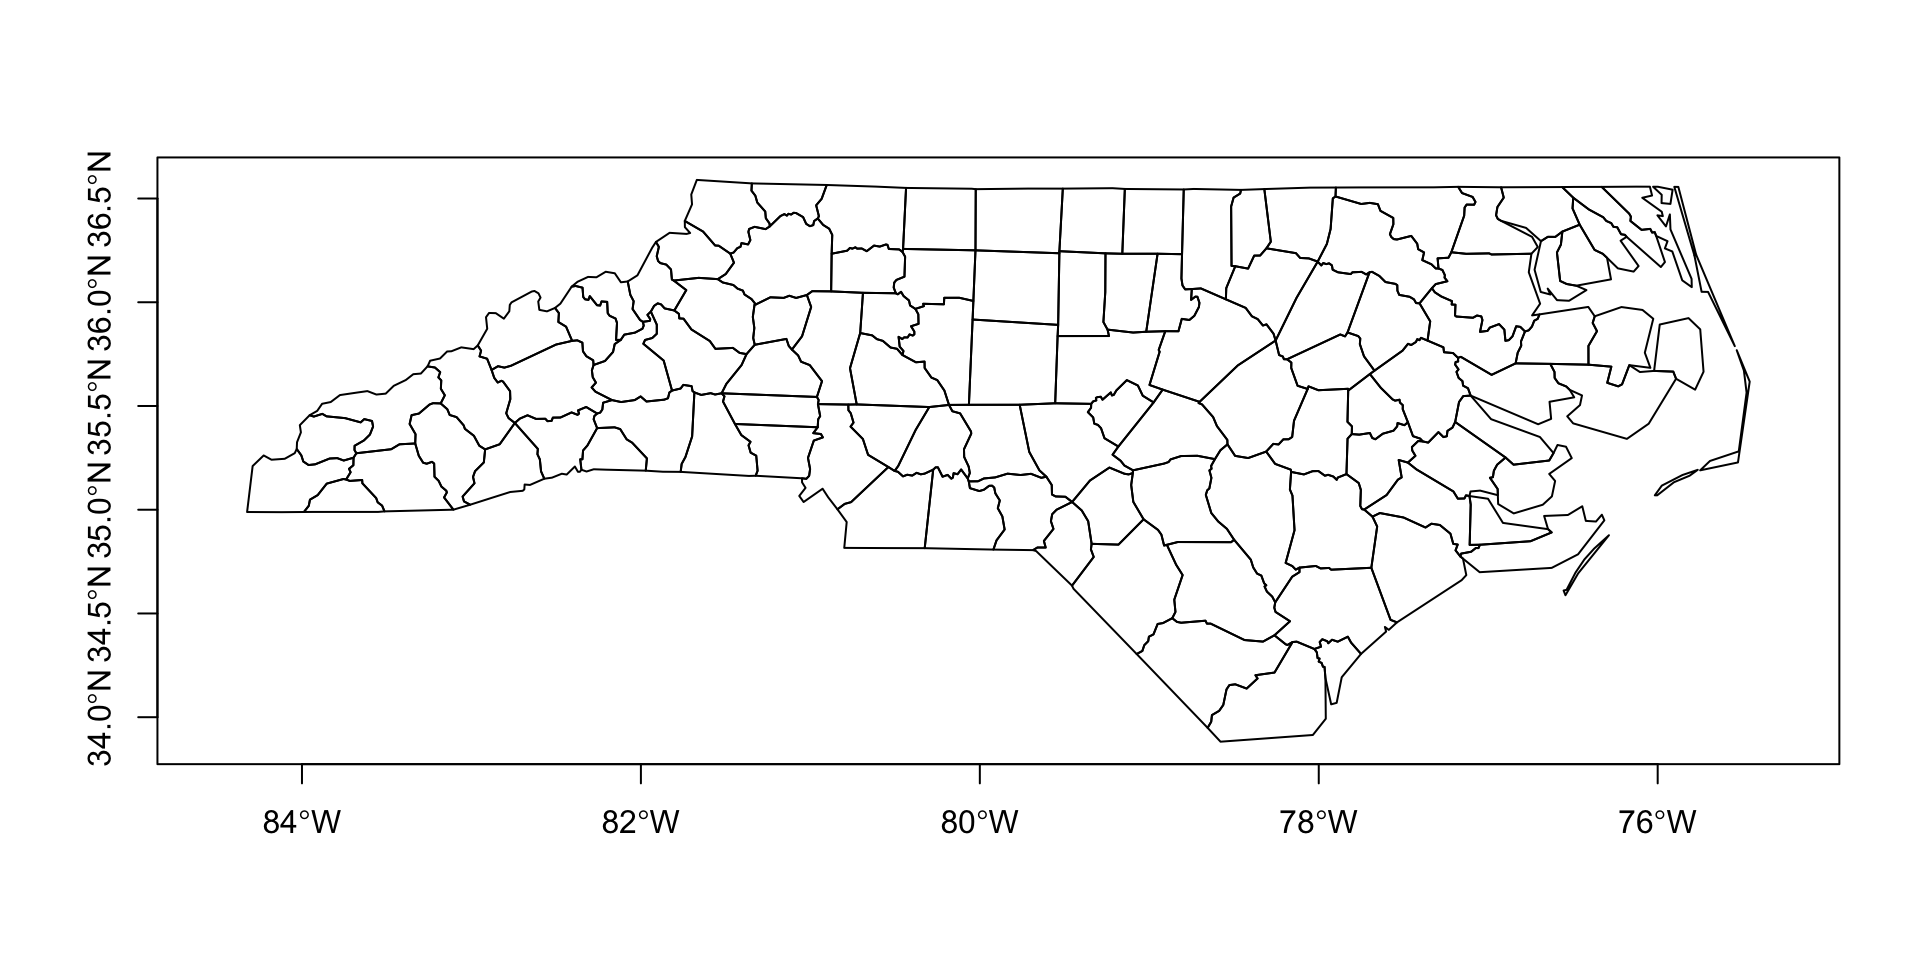
\includegraphics[width=0.8\textwidth]{Lec01_files/figure-beamer/unnamed-chunk-3-1} \end{center}

\end{frame}

\begin{frame}[t]{Least squares fit}
\protect\hypertarget{least-squares-fit}{}

Let \(\hat{\symbf{Y}}\) be our estimate for \(\symbf{Y}\) based on our
estimate of \(\symbf{\beta}\),
\[ \hat{\symbf{Y}} = \hat{\beta}_0 + \hat{\beta}_1 \, \symbf{X}_{1} + \hat{\beta}_2 \, \symbf{X}_{2} + \hat{\beta}_3 \, \symbf{X}_{3} = \symbf{X}\, \hat{\symbf{\beta}} \]

\pause

The least squares estimate, \(\hat{\symbf{\beta}}_{ls}\), is given by
\[ \underset{\symbf{\beta}}{\argmin} \sum_{i=1}^n \left( Y_i - \symbf{X}_{i\cdot} \symbf{\beta} \right)^2 \]

\pause

Previously we derived,
\[ \hat{\symbf{\beta}}_{ls} = (\symbf{X}' \symbf{X})^{-1} \symbf{X}' \, \symbf{Y} \]

\end{frame}

\begin{frame}[fragile,t]{Frequentist Fit}
\protect\hypertarget{frequentist-fit}{}

\begin{Shaded}
\begin{Highlighting}[]
\NormalTok{l =}\StringTok{ }\KeywordTok{lm}\NormalTok{(Y }\OperatorTok{~}\StringTok{ }\NormalTok{X1 }\OperatorTok{+}\StringTok{ }\NormalTok{X2 }\OperatorTok{+}\StringTok{ }\NormalTok{X3, }\DataTypeTok{data=}\NormalTok{d)}
\NormalTok{l}\OperatorTok{$}\NormalTok{coefficients}
\end{Highlighting}
\end{Shaded}

\begin{verbatim}
## (Intercept)          X1          X2          X3 
##   0.6566561   1.4657537  -2.2807109   0.1629704
\end{verbatim}

\begin{Shaded}
\begin{Highlighting}[]
\NormalTok{(}\DataTypeTok{beta_hat =} \KeywordTok{solve}\NormalTok{(}\KeywordTok{t}\NormalTok{(X) }\OperatorTok\StringTok{ }\NormalTok{X, }\KeywordTok{t}\NormalTok{(X)) }\OperatorTok\StringTok{ }\NormalTok{d}\OperatorTok{$}\NormalTok{Y)}
\end{Highlighting}
\end{Shaded}

\begin{verbatim}
##                   [,1]
## (Intercept)  0.6566561
## X1           1.4657537
## X2          -2.2807109
## X3           0.1629704
\end{verbatim}

\end{frame}

\begin{frame}[fragile,t]{Bayesian model specification (JAGS)}
\protect\hypertarget{bayesian-model-specification-jags}{}

\begin{Shaded}
\begin{Highlighting}[]
\NormalTok{model =}\StringTok{ }
\StringTok{"model\{}
\StringTok{  # Likelihood}
\StringTok{  for(i in 1:length(Y))\{}
\StringTok{    Y[i] ~ dnorm(mu[i], tau)}
\StringTok{    mu[i] = beta[1] + beta[2]*X1[i] + beta[3]*X2[i] + beta[4]*X3[i]}
\StringTok{  \}}

\StringTok{  # Prior for beta}
\StringTok{  for(j in 1:4)\{}
\StringTok{    beta[j] ~ dnorm(0,1/100)}
\StringTok{  \}}

\StringTok{  # Prior for sigma / tau2}
\StringTok{  tau ~ dgamma(1, 1)}
\StringTok{  sigma2 = 1/tau}
\StringTok{\}"}
\end{Highlighting}
\end{Shaded}

\end{frame}

\begin{frame}[fragile,t]{Compiling}
\protect\hypertarget{compiling}{}

\scriptsize

\begin{Shaded}
\begin{Highlighting}[]
\NormalTok{m =}\StringTok{ }\NormalTok{rjags}\OperatorTok{::}\KeywordTok{jags.model}\NormalTok{(}
  \KeywordTok{textConnection}\NormalTok{(model), }
  \DataTypeTok{data =}\NormalTok{ d, }\DataTypeTok{n.chains =} \DecValTok{2}
\NormalTok{)}
\end{Highlighting}
\end{Shaded}

\begin{verbatim}
## Compiling model graph
##    Resolving undeclared variables
##    Allocating nodes
## Graph information:
##    Observed stochastic nodes: 100
##    Unobserved stochastic nodes: 5
##    Total graph size: 810
## 
## Initializing model
\end{verbatim}

\end{frame}

\begin{frame}[fragile,t]{Sampling}
\protect\hypertarget{sampling}{}

\begin{Shaded}
\begin{Highlighting}[]
\CommentTok{# Burnin }
\KeywordTok{update}\NormalTok{(m, }\DataTypeTok{n.iter=}\DecValTok{1000}\NormalTok{, }\DataTypeTok{progress.bar=}\StringTok{"none"}\NormalTok{)}

\CommentTok{# Draw samples}
\NormalTok{samp =}\StringTok{ }\NormalTok{rjags}\OperatorTok{::}\KeywordTok{coda.samples}\NormalTok{(}
\NormalTok{  m, }\DataTypeTok{variable.names=}\KeywordTok{c}\NormalTok{(}\StringTok{"beta"}\NormalTok{,}\StringTok{"sigma2"}\NormalTok{), }
  \DataTypeTok{n.iter=}\DecValTok{5000}\NormalTok{, }\DataTypeTok{progress.bar=}\StringTok{"none"}
\NormalTok{)}
\end{Highlighting}
\end{Shaded}

\end{frame}

\begin{frame}[fragile,t]{Results}
\protect\hypertarget{results}{}

\begin{Shaded}
\begin{Highlighting}[]
\KeywordTok{str}\NormalTok{(samp)}
\end{Highlighting}
\end{Shaded}

\begin{verbatim}
## List of 2
##  $ : 'mcmc' num [1:5000, 1:5] 0.477 0.533 0.513 0.608 0.47 ...
##   ..- attr(*, "dimnames")=List of 2
##   .. ..$ : NULL
##   .. ..$ : chr [1:5] "beta[1]" "beta[2]" "beta[3]" "beta[4]" ...
##   ..- attr(*, "mcpar")= num [1:3] 1001 6000 1
##  $ : 'mcmc' num [1:5000, 1:5] 0.729 0.351 0.576 0.687 0.622 ...
##   ..- attr(*, "dimnames")=List of 2
##   .. ..$ : NULL
##   .. ..$ : chr [1:5] "beta[1]" "beta[2]" "beta[3]" "beta[4]" ...
##   ..- attr(*, "mcpar")= num [1:3] 1001 6000 1
##  - attr(*, "class")= chr "mcmc.list"
\end{verbatim}

\end{frame}

\begin{frame}[fragile,t]{CODA \& mcmc objects}
\protect\hypertarget{coda-mcmc-objects}{}

\begin{Shaded}
\begin{Highlighting}[]
\KeywordTok{head}\NormalTok{(samp[[}\DecValTok{1}\NormalTok{]])}
\end{Highlighting}
\end{Shaded}

\begin{verbatim}
## Markov Chain Monte Carlo (MCMC) output:
## Start = 1001 
## End = 1007 
## Thinning interval = 1 
##        beta[1]  beta[2]   beta[3]    beta[4]    sigma2
## [1,] 0.4772517 1.419778 -2.199144 0.28649330 1.0809728
## [2,] 0.5328665 1.521434 -2.391340 0.10170084 1.2145136
## [3,] 0.5127307 1.569942 -2.288688 0.09279966 1.2330530
## [4,] 0.6082786 1.457989 -2.301124 0.11507748 0.7760024
## [5,] 0.4696911 1.497949 -2.427537 0.15902657 1.1581875
## [6,] 0.7505117 1.397314 -2.231748 0.04573775 0.9684167
## [7,] 0.6361385 1.625917 -2.208012 0.21898668 1.3867957
\end{verbatim}

\end{frame}

\begin{frame}[fragile,t]{CODA \& mcmc objects - plotting}
\protect\hypertarget{coda-mcmc-objects---plotting}{}

\begin{Shaded}
\begin{Highlighting}[]
\KeywordTok{plot}\NormalTok{(samp)}
\end{Highlighting}
\end{Shaded}

\begin{center}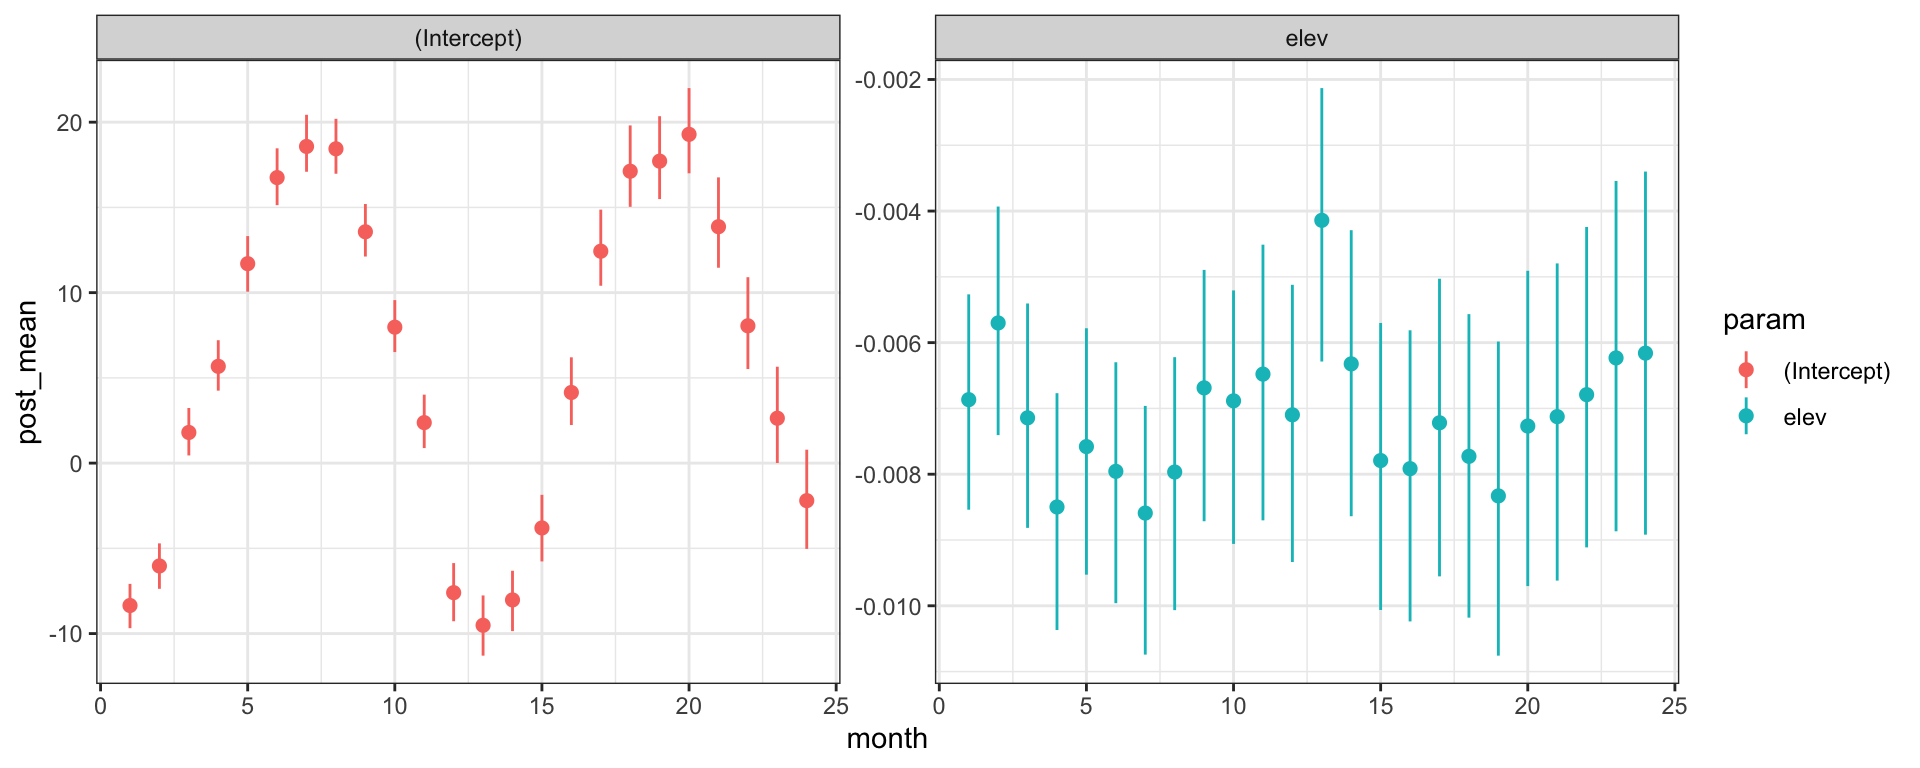
\includegraphics[width=\textwidth]{Lec01_files/figure-beamer/unnamed-chunk-10-1} \end{center}

\begin{center}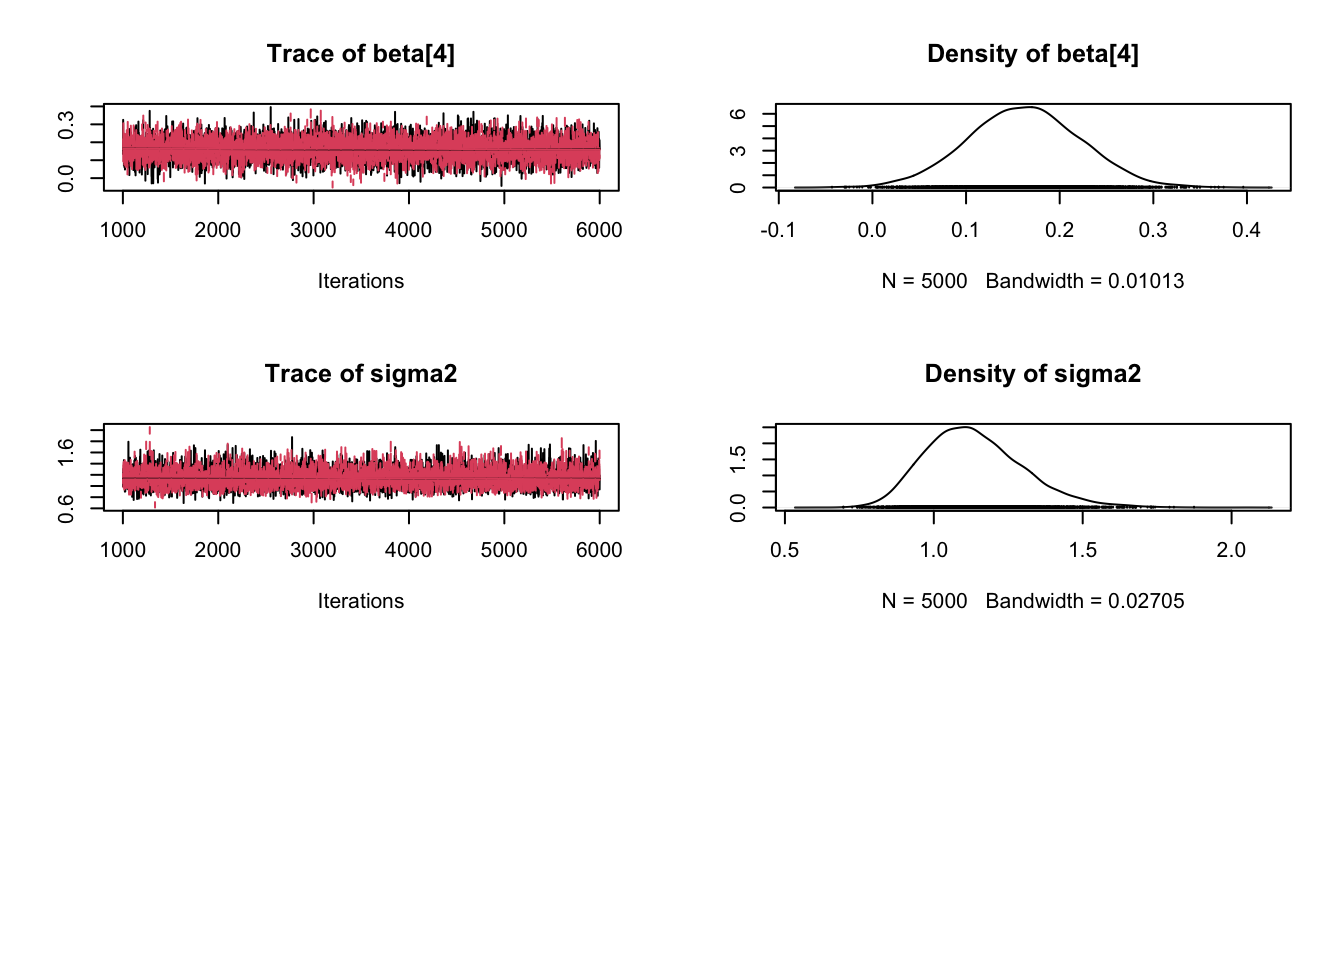
\includegraphics[width=\textwidth]{Lec01_files/figure-beamer/unnamed-chunk-10-2} \end{center}

\end{frame}

\begin{frame}[fragile,t]{Tidy Bayes}
\protect\hypertarget{tidy-bayes}{}

\begin{Shaded}
\begin{Highlighting}[]
\NormalTok{df =}\StringTok{ }\NormalTok{samp }\OperatorTok
\StringTok{  }\NormalTok{tidybayes}\OperatorTok{::}\KeywordTok{gather_draws}\NormalTok{(beta[i], sigma2) }\OperatorTok
\StringTok{  }\KeywordTok{mutate}\NormalTok{(}\DataTypeTok{param =} \KeywordTok{ifelse}\NormalTok{(}\KeywordTok{is.na}\NormalTok{(i), .variable, }\KeywordTok{paste0}\NormalTok{(.variable,}\StringTok{"["}\NormalTok{,i,}\StringTok{"]"}\NormalTok{)))}

\NormalTok{df}
\end{Highlighting}
\end{Shaded}

\begin{verbatim}
## # A tibble: 50,000 x 7
## # Groups:   i, .variable [5]
##    .chain .iteration .draw     i .variable .value param  
##     <int>      <int> <int> <int> <chr>      <dbl> <chr>  
##  1      1          1     1     1 beta       0.477 beta[1]
##  2      1          1     1     2 beta       1.42  beta[2]
##  3      1          1     1     3 beta      -2.20  beta[3]
##  4      1          1     1     4 beta       0.286 beta[4]
##  5      1          2     2     1 beta       0.533 beta[1]
##  6      1          2     2     2 beta       1.52  beta[2]
##  7      1          2     2     3 beta      -2.39  beta[3]
##  8      1          2     2     4 beta       0.102 beta[4]
##  9      1          3     3     1 beta       0.513 beta[1]
## 10      1          3     3     2 beta       1.57  beta[2]
## # ... with 49,990 more rows
\end{verbatim}

\end{frame}

\begin{frame}[fragile,t]{Tidy Bayes + ggplot - Traceplot}
\protect\hypertarget{tidy-bayes-ggplot---traceplot}{}

\scriptsize

\begin{Shaded}
\begin{Highlighting}[]
\KeywordTok{ggplot}\NormalTok{(df, }\KeywordTok{aes}\NormalTok{(}\DataTypeTok{x=}\NormalTok{.iteration, }\DataTypeTok{y=}\NormalTok{.value, }\DataTypeTok{color=}\KeywordTok{as.character}\NormalTok{(.chain))) }\OperatorTok{+}
\StringTok{  }\KeywordTok{geom_line}\NormalTok{(}\DataTypeTok{alpha=}\FloatTok{0.5}\NormalTok{) }\OperatorTok{+}
\StringTok{  }\KeywordTok{facet_wrap}\NormalTok{(}\OperatorTok{~}\NormalTok{param, }\DataTypeTok{scale=}\StringTok{"free_y"}\NormalTok{) }\OperatorTok{+}
\StringTok{  }\KeywordTok{labs}\NormalTok{(}\DataTypeTok{color=}\StringTok{"Chain"}\NormalTok{)}
\end{Highlighting}
\end{Shaded}

\begin{center}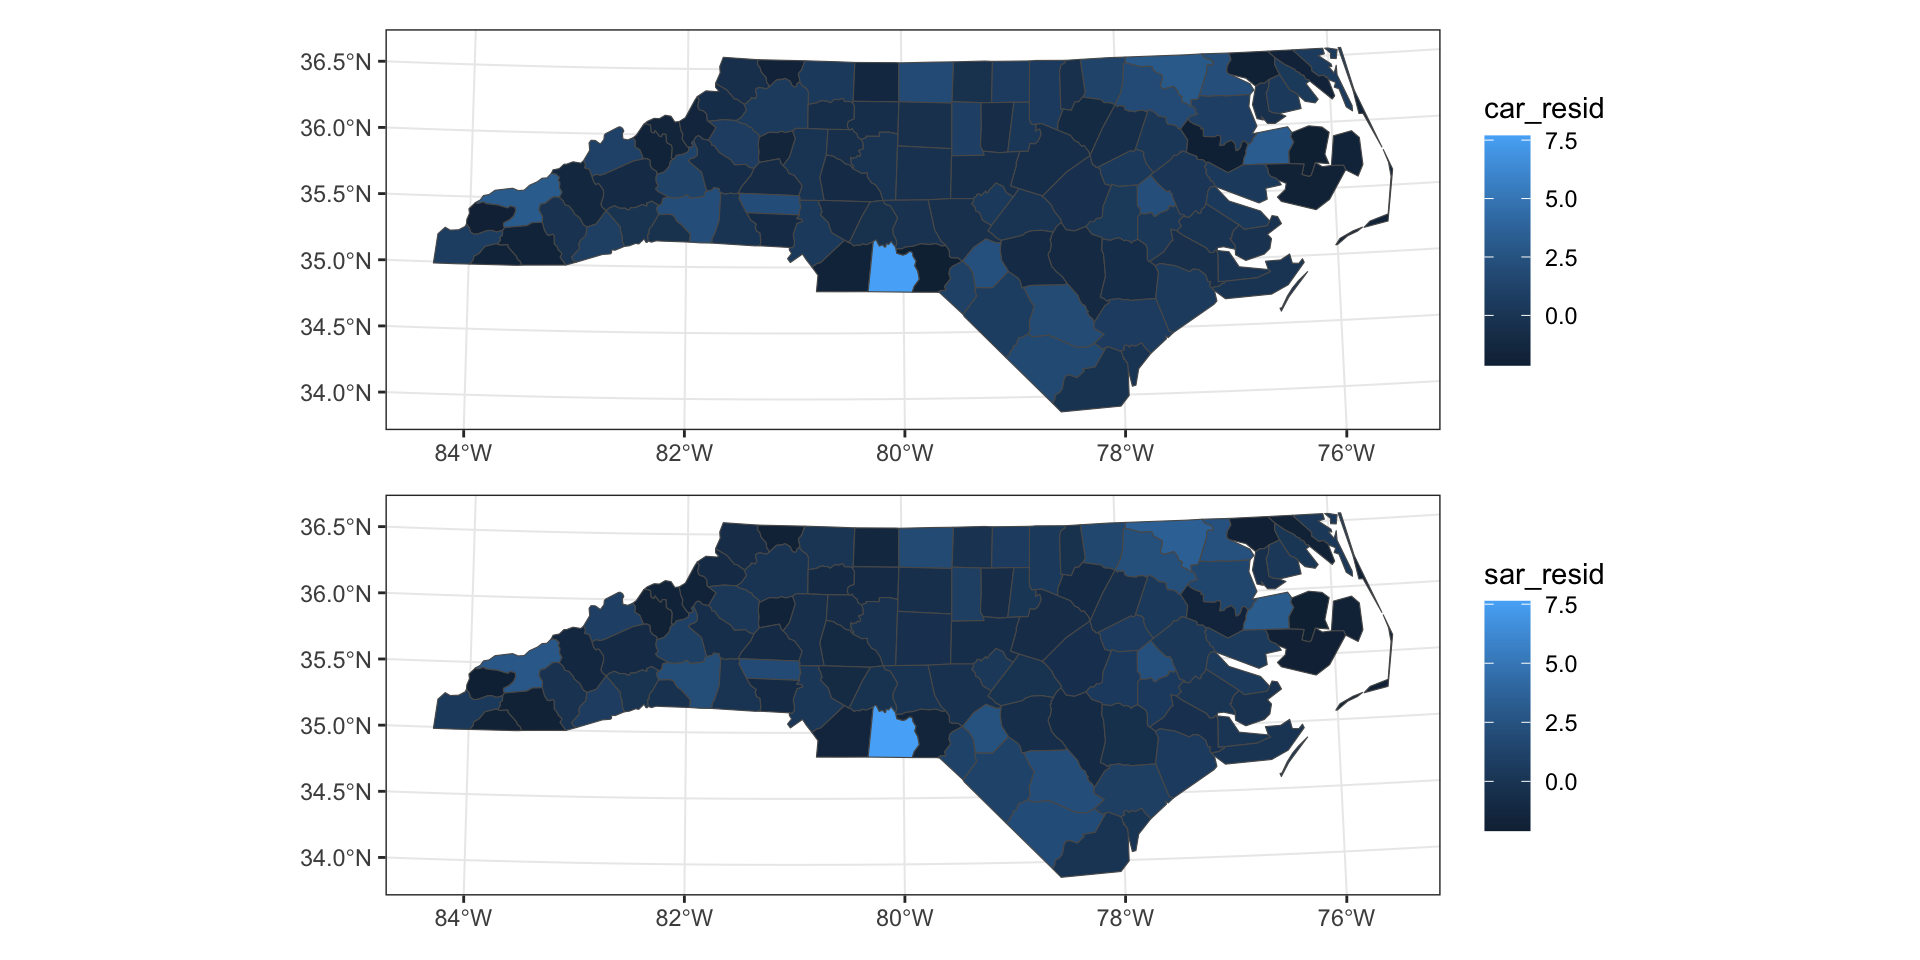
\includegraphics[width=\textwidth]{Lec01_files/figure-beamer/unnamed-chunk-12-1} \end{center}

\end{frame}

\begin{frame}[fragile,t]{Tidy Bayes + ggplot - Density plot}
\protect\hypertarget{tidy-bayes-ggplot---density-plot}{}

\scriptsize

\begin{Shaded}
\begin{Highlighting}[]
\KeywordTok{ggplot}\NormalTok{(df, }\KeywordTok{aes}\NormalTok{(}\DataTypeTok{x=}\NormalTok{.value, }\DataTypeTok{fill=}\KeywordTok{as.character}\NormalTok{(.chain))) }\OperatorTok{+}
\StringTok{  }\KeywordTok{geom_density}\NormalTok{(}\DataTypeTok{alpha=}\FloatTok{0.5}\NormalTok{) }\OperatorTok{+}
\StringTok{  }\KeywordTok{facet_wrap}\NormalTok{(}\OperatorTok{~}\NormalTok{param, }\DataTypeTok{scale=}\StringTok{"free_x"}\NormalTok{) }\OperatorTok{+}
\StringTok{  }\KeywordTok{labs}\NormalTok{(}\DataTypeTok{fill=}\StringTok{"Chain"}\NormalTok{)}
\end{Highlighting}
\end{Shaded}

\begin{center}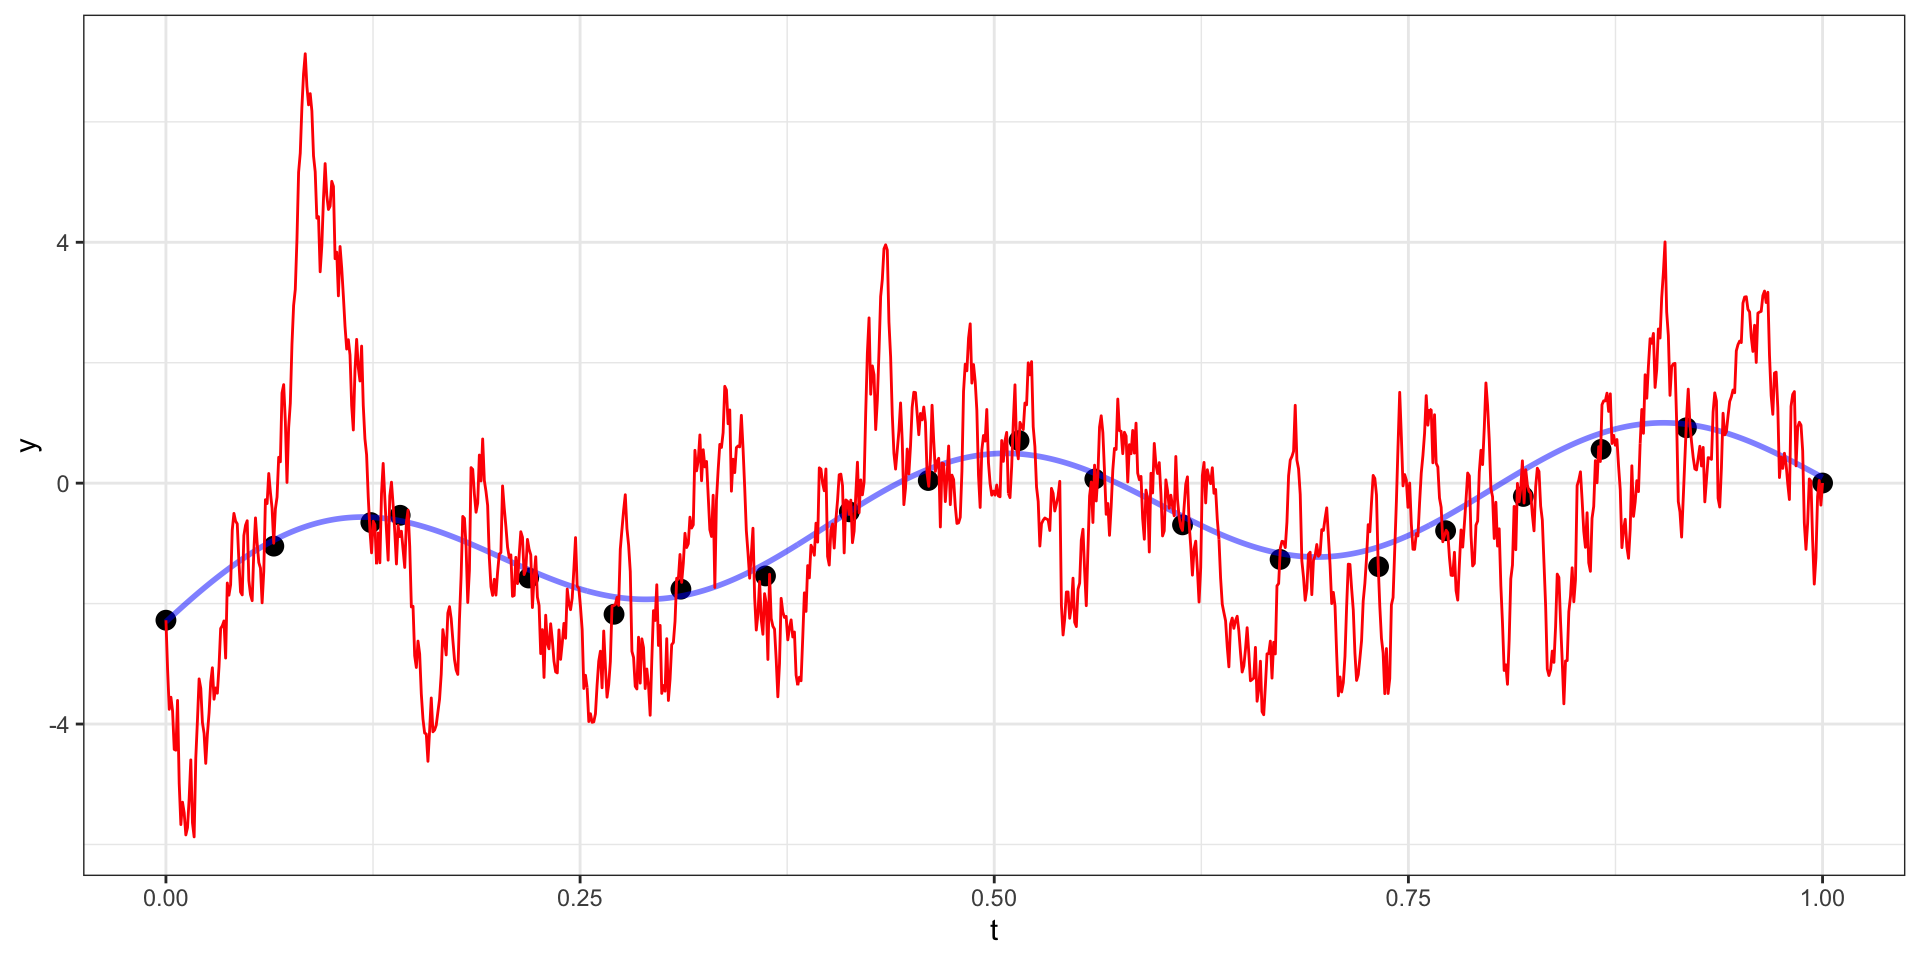
\includegraphics[width=\textwidth]{Lec01_files/figure-beamer/unnamed-chunk-13-1} \end{center}

\end{frame}

\begin{frame}[fragile]{Comparing Approaches}
\protect\hypertarget{comparing-approaches}{}

\scriptsize

\begin{Shaded}
\begin{Highlighting}[]
\NormalTok{pt_est =}\StringTok{ }\NormalTok{df }\OperatorTok\StringTok{ }
\StringTok{  }\KeywordTok{filter}\NormalTok{(.chain }\OperatorTok{==}\StringTok{ }\DecValTok{1}\NormalTok{) }\OperatorTok
\StringTok{  }\KeywordTok{group_by}\NormalTok{(param) }\OperatorTok\StringTok{ }
\StringTok{  }\KeywordTok{summarize}\NormalTok{(}\DataTypeTok{post_mean =} \KeywordTok{mean}\NormalTok{(.value)) }\OperatorTok
\StringTok{  }\KeywordTok{ungroup}\NormalTok{() }\OperatorTok
\StringTok{  }\KeywordTok{mutate}\NormalTok{(}
    \DataTypeTok{truth =} \KeywordTok{c}\NormalTok{(}\FloatTok{0.7}\NormalTok{, }\FloatTok{1.5}\NormalTok{, }\FloatTok{-2.2}\NormalTok{, }\FloatTok{0.1}\NormalTok{, }\DecValTok{1}\NormalTok{),}
    \DataTypeTok{ols   =} \KeywordTok{c}\NormalTok{(l}\OperatorTok{$}\NormalTok{coefficients, }\KeywordTok{var}\NormalTok{(l}\OperatorTok{$}\NormalTok{residuals))}
\NormalTok{  ) }\OperatorTok
\StringTok{  }\KeywordTok{select}\NormalTok{(param, truth, ols, post_mean)}

\NormalTok{pt_est}
\end{Highlighting}
\end{Shaded}

\begin{verbatim}
## # A tibble: 5 x 4
##   param   truth    ols post_mean
##   <chr>   <dbl>  <dbl>     <dbl>
## 1 beta[1]   0.7  0.657     0.656
## 2 beta[2]   1.5  1.47      1.47 
## 3 beta[3]  -2.2 -2.28     -2.28 
## 4 beta[4]   0.1  0.163     0.164
## 5 sigma2    1    1.08      1.14
\end{verbatim}

\end{frame}

\begin{frame}[fragile,t]{Comparing Approaches - code}
\protect\hypertarget{comparing-approaches---code}{}

\begin{Shaded}
\begin{Highlighting}[]
\KeywordTok{ggplot}\NormalTok{(df, }\KeywordTok{aes}\NormalTok{(}\DataTypeTok{x=}\NormalTok{.value, }\DataTypeTok{fill=}\KeywordTok{as.character}\NormalTok{(.chain))) }\OperatorTok{+}
\StringTok{  }\KeywordTok{geom_density}\NormalTok{(}\DataTypeTok{alpha=}\FloatTok{0.5}\NormalTok{) }\OperatorTok{+}
\StringTok{  }\KeywordTok{facet_wrap}\NormalTok{(}\OperatorTok{~}\NormalTok{param, }\DataTypeTok{scale=}\StringTok{"free_x"}\NormalTok{) }\OperatorTok{+}
\StringTok{  }\KeywordTok{geom_vline}\NormalTok{(}
    \DataTypeTok{data =}\NormalTok{ tidyr}\OperatorTok{::}\KeywordTok{gather}\NormalTok{(pt_est, pt_est, value, }\OperatorTok{-}\NormalTok{param), }
    \KeywordTok{aes}\NormalTok{(}\DataTypeTok{xintercept =}\NormalTok{ value, }\DataTypeTok{color=}\NormalTok{pt_est)}
\NormalTok{  ) }\OperatorTok{+}
\StringTok{  }\KeywordTok{labs}\NormalTok{(}\DataTypeTok{fill=}\StringTok{"Chain"}\NormalTok{)}
\end{Highlighting}
\end{Shaded}

\end{frame}

\begin{frame}[t]{Comparing Approaches - plot}
\protect\hypertarget{comparing-approaches---plot}{}

\begin{center}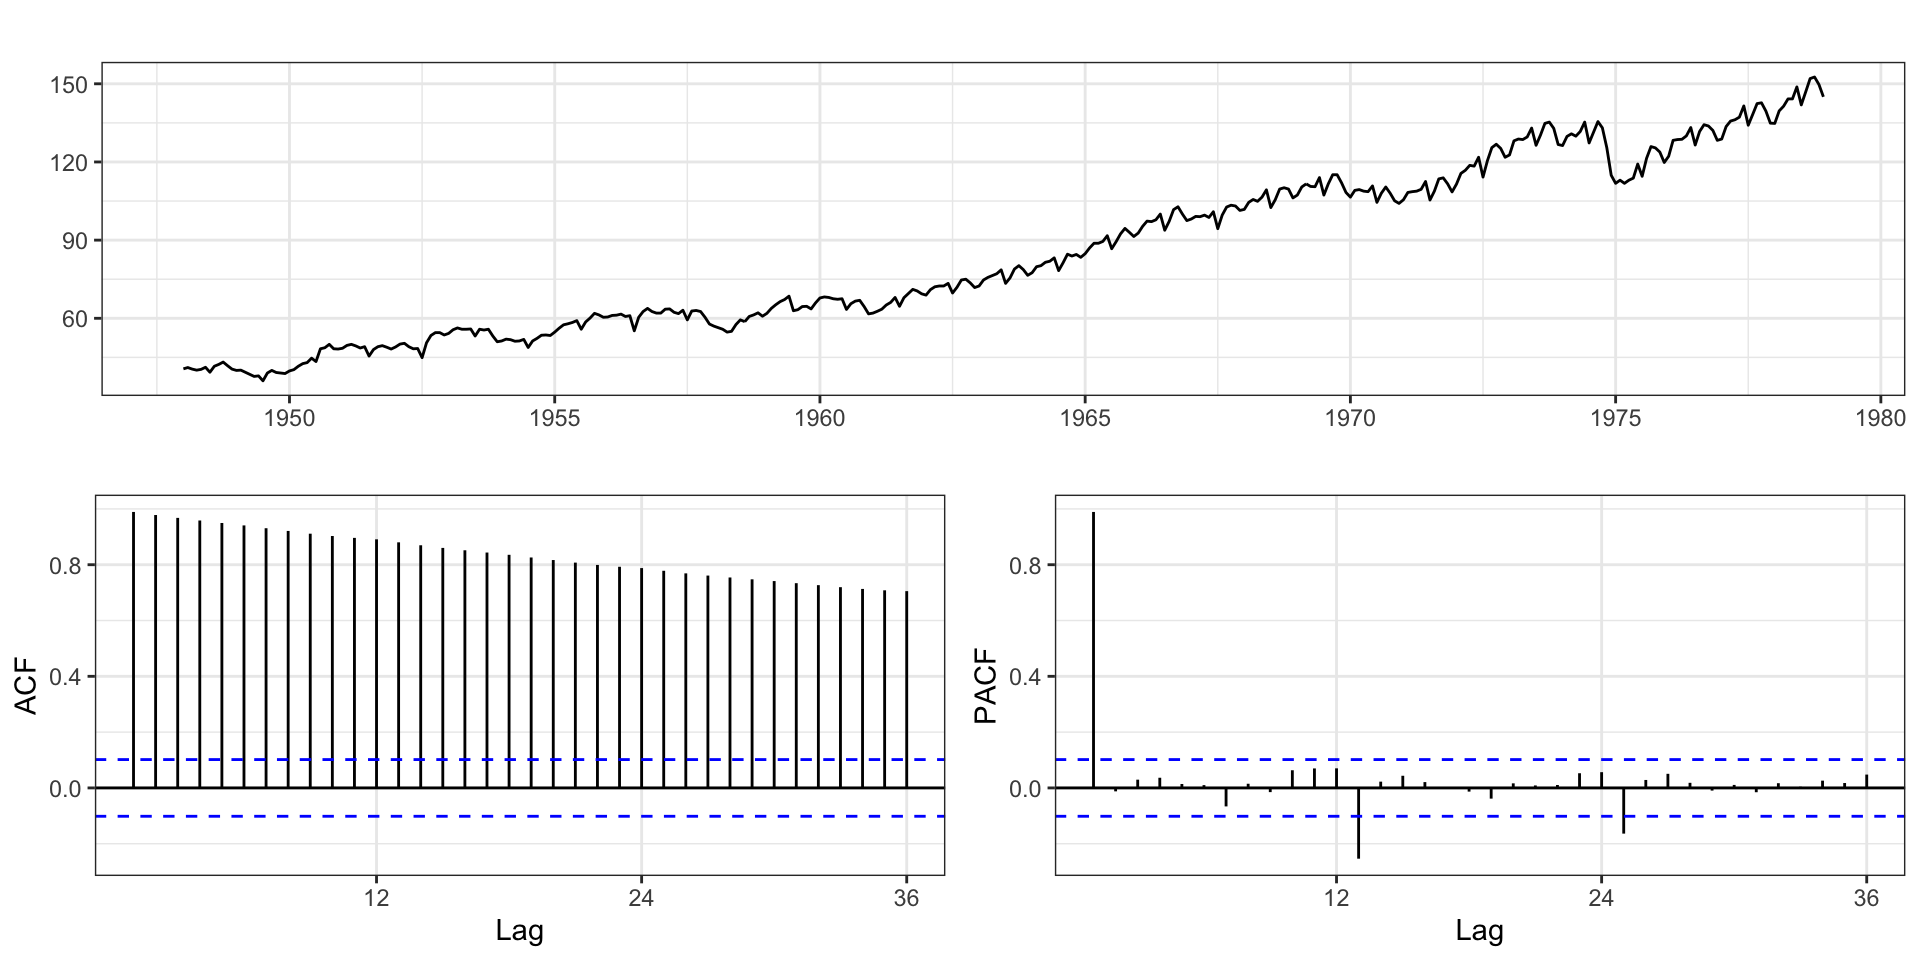
\includegraphics[width=\textwidth]{Lec01_files/figure-beamer/unnamed-chunk-15-1} \end{center}

\end{frame}

\end{document}
